\documentclass{report}
\usepackage[utf8]{inputenc}
\usepackage[francais]{babel}
\usepackage[T1]{fontenc}
\usepackage{graphicx}
\usepackage{multicol}
\usepackage{ stmaryrd }

\title{Projet IHM \\ TAGulous}
\author{David Kerbrat et Ygor Gallina}
\date{March 2017}

\begin{document}

\maketitle

\tableofcontents

\chapter{Introduction}

    L'objectif de ce projet est de créer une application de bureau permettant de tagguer des fichiers et des dossiers. Un tag est un mot-clé associé à des fichiers ou des dossiers permettant de les classer indépendament du systéme de fichier hierarchique. Notre application est prévue pour tourner sous macOS (testée sous macOS Sierra).\\
    
    Notre application s'adresse à des utilisateur-trices déjà familiarisés avec l'outil informatiques mais ne requiert pas de connaissance particulière.\\

\chapter{Évolution du projet}

    Au cours de notre réflexion, nous nous sommes confrontés à différents choix d'interface et de fonctionnalités qui nous ont amenés à améliorer ou réviser notre projet, jusqu'à aboutir à une version finale qui est celle sur laquelle nous sommes partis pour l'implémenter.

    \section{Première version}
            \begin{figure}[htbp]
            \begin{center}
                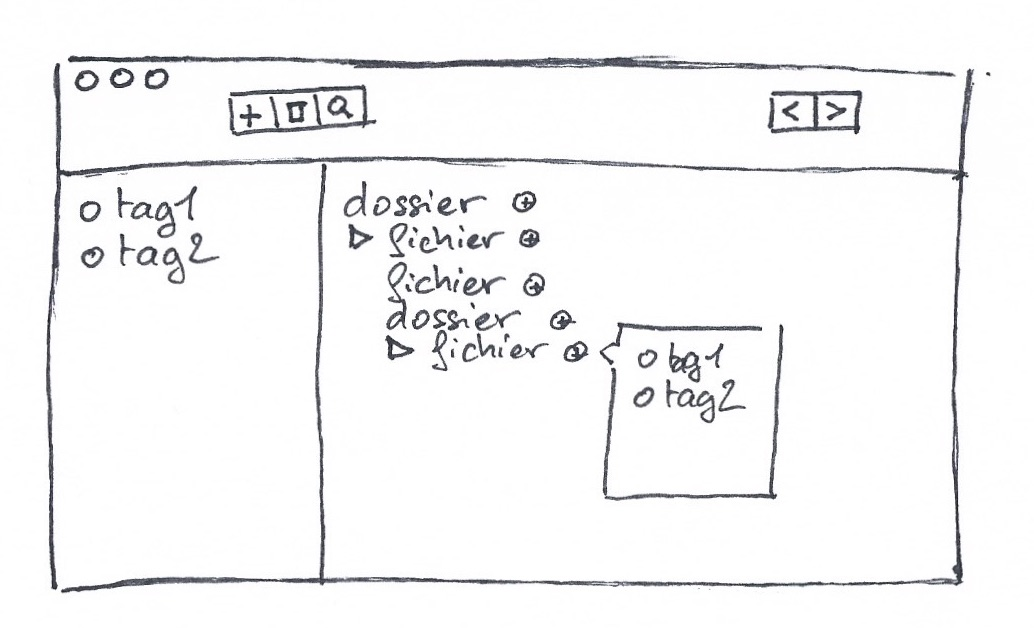
\includegraphics[width=10cm]{version1.jpg}
                \caption{paper prototype de la première version, en mode tagging}
                \end{center}
            \end{figure}
        \subsection{Présentation de l'idée}
            Pour la première version, nous nous sommes inspiré du Finder de Apple qui permet de tagguer nos fichiers et dossiers sur macOS. Nous avons donc imaginé une interface scindée en deux parties : la première sur la gauche présente une liste des tags et la seconde à droite, plus grande, contient soit un explorateur de fichier lorsque l'on est en mode "tagging", soit une liste de fichiers taggués lorsque l'on est en mode "recherche/filtrage".\\
        
            

            Dans cette version, le tagging s'effectue grâce à des petits boutons situés à droite des noms de dossiers et fichiers dans le volet explorateur. Il permettent de choisir le ou les tag-s au-x-quel-s on veut attacher le fichier ou le dossier, en leur permettant d'avoir plusieurs tags.\\

            La visualisation des fichiers et dossiers taggués et le filtrage s'effectue en cliquant sur le nom d'un tag dans la liste de gauche. Le panneau contenant l'explorateur affiche alors la liste des fichiers tagués. En selectionnant plusieurs tag (en maintenant la touche Maj enfoncée ou en cliquant sur l'icône filtrage/recherche symbolisé par une loupe) on obtient la liste des fichier ayant l'un ou l'autre des tags.

        \subsection{Les limites de cette version}

            Le principal défaut que l'on a trouvé à cette version, c'est la redondance et le manque d'intégration dans le système. En effet, l'utilisateur-trice dispose d'un explorateur de fichier classique et d'un explorateur de fichier au sein de l'application. L'aller-retour entre l'un et l'autre manque donc de fluidité. Nous avons donc modifié notre idée pour arriver à la deuxième version.

    \section{Deuxième version}
            \begin{figure}[htbp]
            \begin{center}
                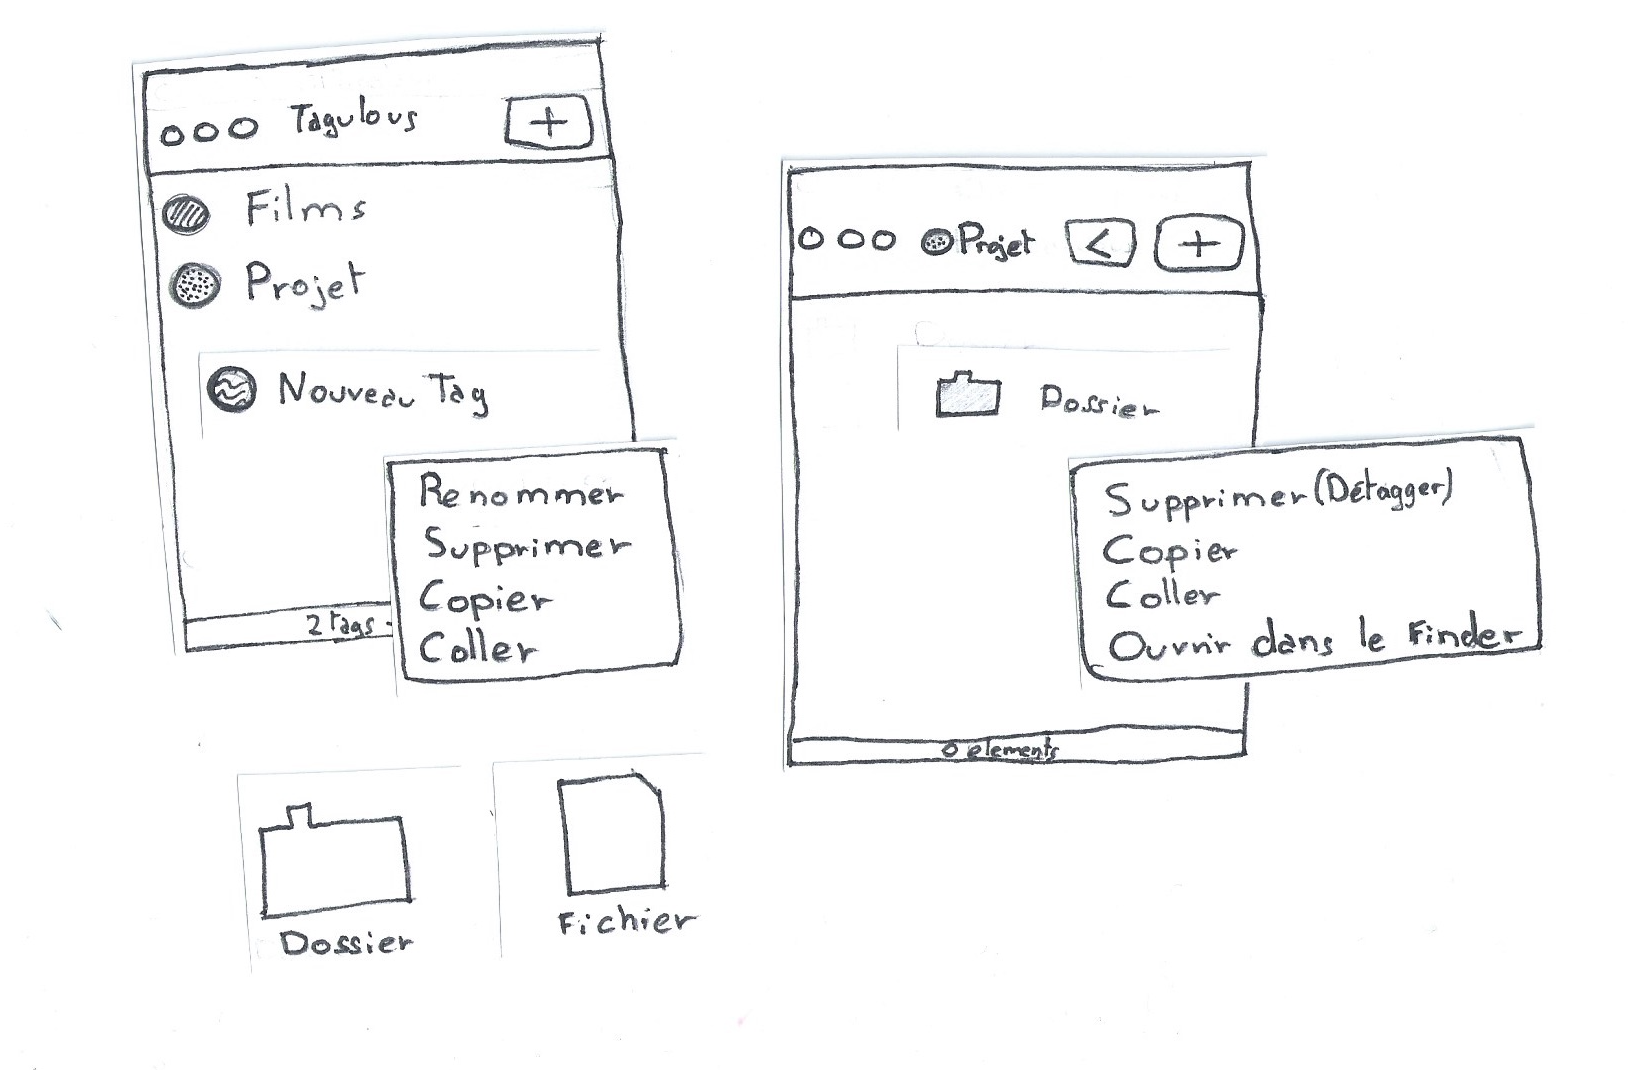
\includegraphics[width=10cm]{version2.png}
                \caption{paper prototype de la deuxième version, à gauche en mode tagging et à droite en visualisation}
                \end{center}
            \end{figure}
        \subsection{Présentation de l'idée}
            Nous avons eu l'idée de simplifier l'application à une simble liste de tags, que l'on utilise en parallèle de l'explorateur de fichier. L'application se présente donc volontairement sous une forme minimaliste et intuitive en reprenant les habitudes de l'utilisateur-trice.\\
            
            Dans cette version, l'application se présente sous la forme d'une liste de tag sur lesquels il suffit de glisser le fichier ou le dossier que l'on veut taguer. On peut ajouter des tags grâce au bouton +. Les fonctionnalités moins fréquentes (supprimer, renommer, etc.) sont accessibles via le menu contextuel. Grâce à cette méthode on réduit drastiquement le nombre de clics nécéssaires pour taguer un fichier.\\
            
            Pour visualiser la liste des fichier tagués, il faut cliquer sur le nom du tag et on obtient la liste désirée. Le bouton + permet d'ajouter un fichier ou un dossier au tag, le bouton < permet de revenir à la liste des tags. Là encore, les actions moins fréquentes sont accessibles via le menu contextuel. Il est possible d'ouvrir le fichier ou le dossier dans l'explorateur du système.\\
            
            Nous avons également pensé pour cette version à transformer la liste des tags en volet qui puisse s'afficher par dessus la liste des fichiers, mais l'idée ne nous a finalement pas parue pertinente.\\
            
            L'application possède aussi une barre d'informations en bas de la fenêtre, qui indique le nombre d'éléments dans la vue courante (c'est-à-dire le nombre de tags ou le nombre de fichiers et dossiers).\\
            
        \subsection{Les limites de cette version}
            Le principal problème rencontré au cours de nos tests est l'impossibilité de filtrer les fichiers et dossiers de façon à obtenir la liste des fichiers correspondants à plusieurs tags. C'est ce problème que nous avons cherché à résoudre dans la version finale.
            
            
    \section{Version finale}
    
        \subsection{Présentation de l'idée}
            Pour cette version, nous avons repris le travail précédant en ajoutant un mode : le mode filtrage. Ce mode permet de choisir d'afficher plusieurs tags en même temps, grâce à un système de checkbox.
            
            \begin{figure}[htbp]
            \begin{center}
                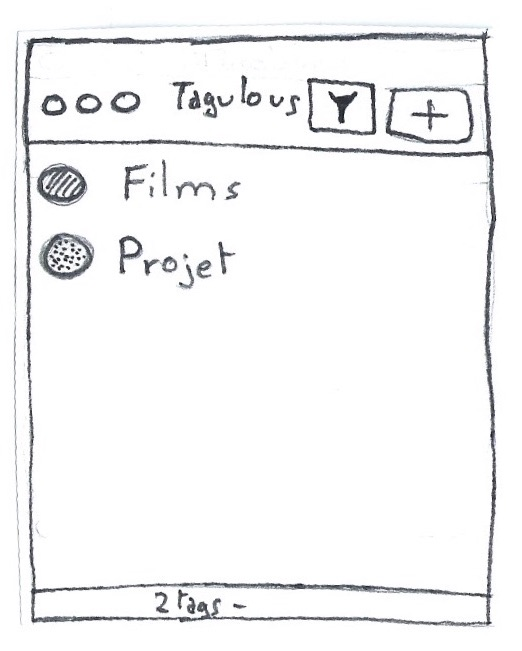
\includegraphics[width=4cm]{version3bis.jpg}
                \caption{paper prototype du mode liste de tags avec le bouton filtre}
                \end{center}
            \end{figure}
            
            À l'usage, il suffit de passer en mode filtrage et de cocher les tags que l'ont veut visualiser. La fenêtre suivante nous affiche tous les fichiers et dossiers tagués (l'union des tags selectionnés, et non l'intersection).
            
            \begin{figure}[htbp]
            \begin{center}
                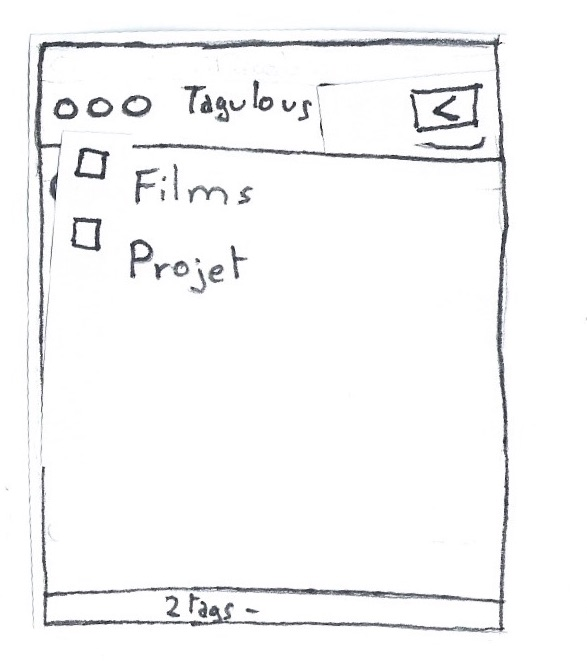
\includegraphics[width=4cm]{version3.jpg}
                \caption{paper prototype du mode filtrage}
                \end{center}
            \end{figure}            

\chapter{Implémentation avec Qt}
    \section{Fonctionnement de l'application}
        L'application reprend donc les principes de la version finale du paper prototype. Elle se divise en trois modes : le mode liste de tags, le mode visualisation des fichiers et le mode filtrage. Elle s'ouvre sur le mode liste de tags qui est l'écran principal de l'application.
        \begin{figure}[htbp]
            \begin{center}
            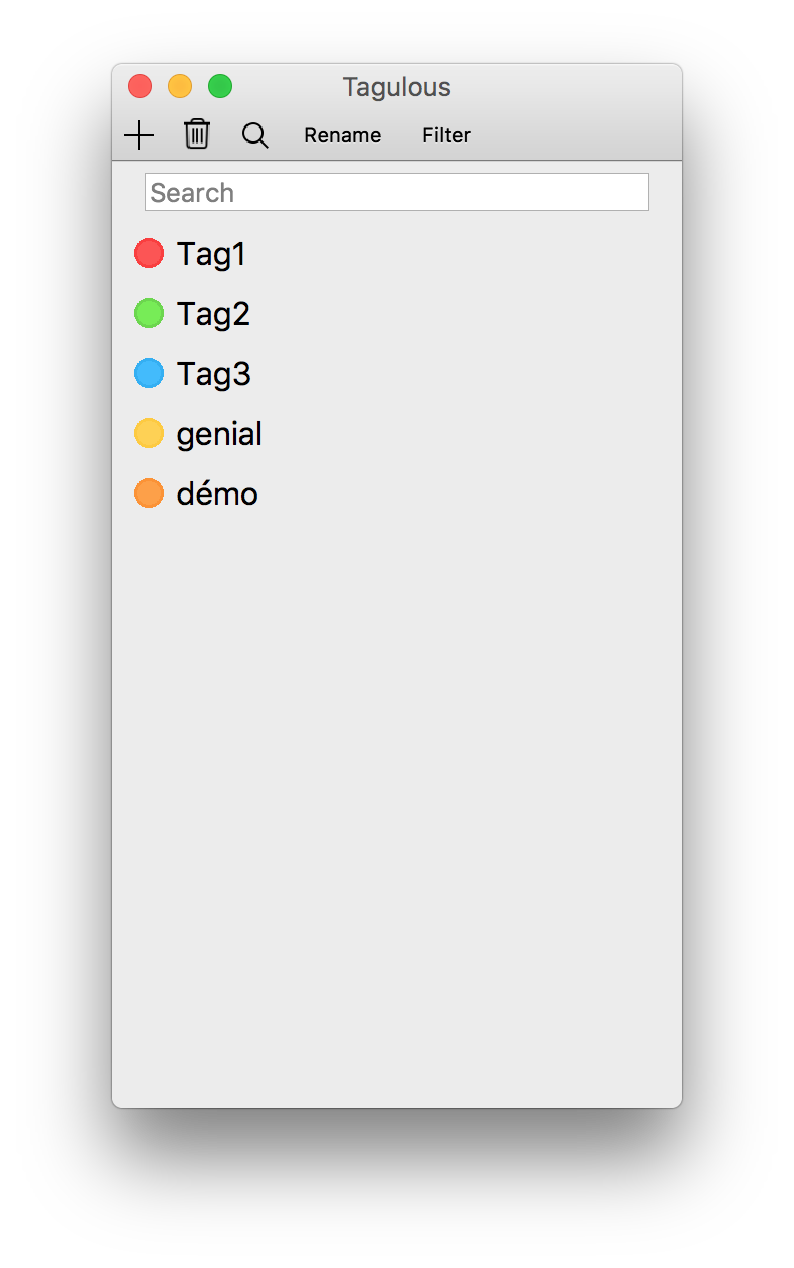
\includegraphics[width=4cm]{listetags.png}
            \caption{Fenêtre principale en mode liste de tags}
            \end{center}
        \end{figure}
    
    Dans le mode liste de tags, on peut ajouter, supprimer ou renommer des tags grâce aux boutons présents dans la barre d'outils ou grâce aux raccourcis habituels, connus de l'utilisateur-trice : Cmd+N pour créer un nouveau tag, double-clic long pour renommer et $\shortleftarrow$ pour supprimer. Chaque tag est identifié par une couleur et un nom. Il est également possible de rechercher un tag en utilisant la barre de recherche (en pratique, cette fonctionnalité ne marche pas car le \texttt{QSortFilterProxyModel} de Qt semble buggué).\\
    
    Pour taguer un fichier ou un dossier, il suffit de le glisser déposer sur le nom du tag voulu. Les noms des tags sont écris dans une police plutôt grande pour respecter la loi de Fitt : le rapport entre la taille de la cible et la distance depuis la source du glisser-déposer qui est souvent grande.
        \begin{figure}[htbp]
            \begin{center}
            \includegraphics[width=10cm]{glisserdeposer.png}
            \caption{Glisser-déposer d'un fichier sur un tag}
            \end{center}
        \end{figure}
    \\
    On accède aux fichiers à partir de liste de tags en double cliquant sur le nom ou la pastille de couleur du tag.\\
        \begin{figure}[htbp]
            \begin{center}
            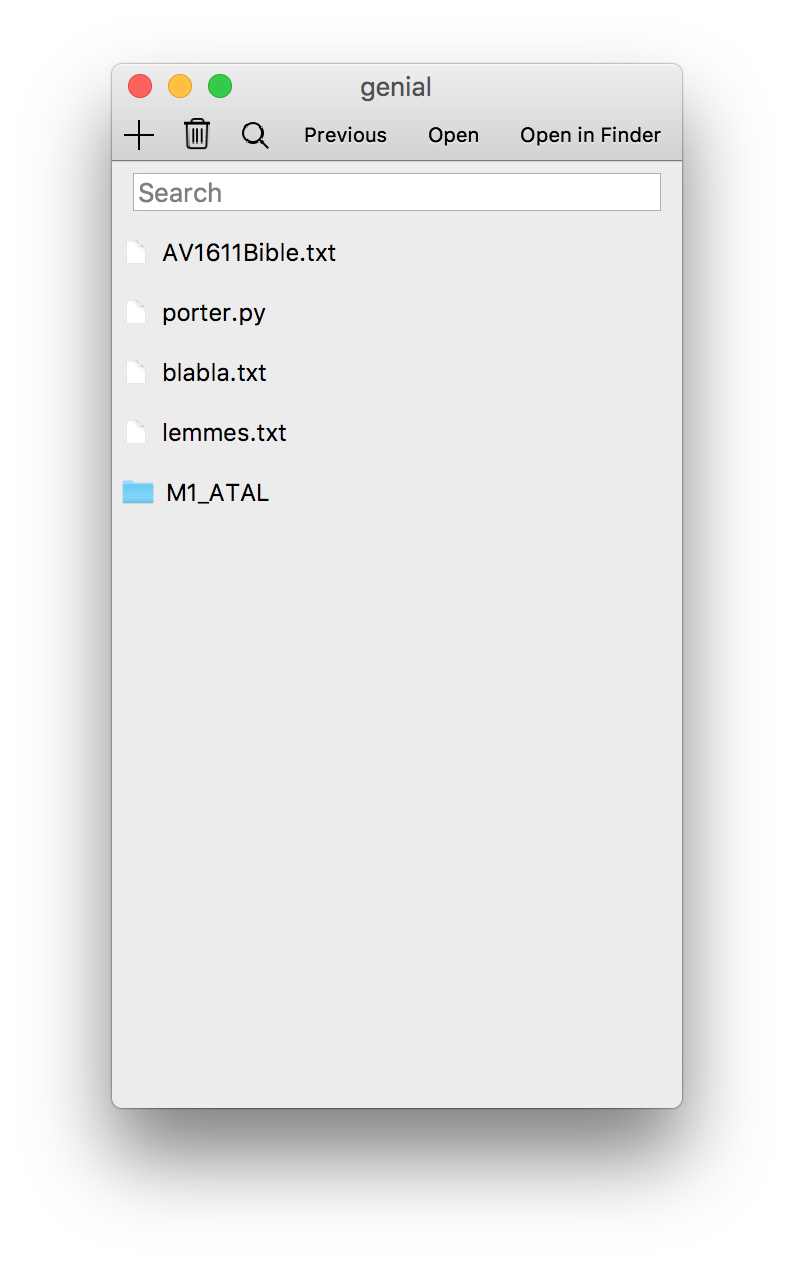
\includegraphics[width=4cm]{listefichiers.png}
            \caption{Mode liste des fichiers associés à un tag}
            \end{center}
        \end{figure}
        
    On obtient la liste des fichiers et dossier associés aux tags, dont le nom est rappelé dans le titre de la fenêtre. Il possible comme dans le mode liste de tags de supprimer des fichiers ou dossiers, d'en ajouter grâce au bouton +, au raccourci Cmd+N ou de manière plus intuitive par un glisser-déposer de un ou plusieurs fichiers ou dossiers. Double cliquer sur un fichier permet de l'ouvrir, et le bouton "Open in Finder" permet de l'afficher dans l'explorateur de fichier. Le bouton "Previous" permet de revenir à l'écran précédent.\\
    
    Sur l'écran principal (liste des tags), on accède à la fonction de filtrage en appuyant sur le bouton "Filtre".\\
    
    \begin{figure}[htbp]
            \begin{center}
            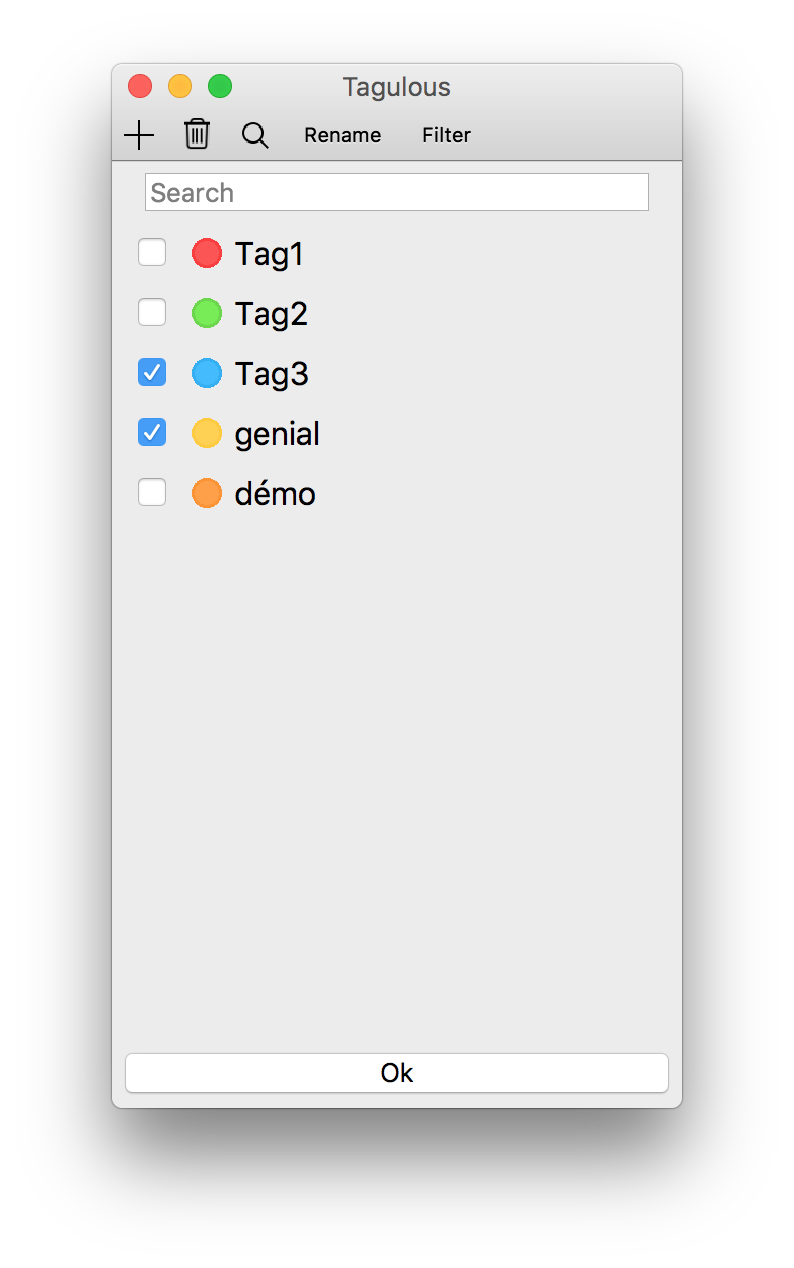
\includegraphics[width=4cm]{modefiltre.png}
            \caption{Mode liste des fichiers associés à un tag}
            \end{center}
        \end{figure}
    
    A partir de cet écran, on peut cocher les tags que l'on veut afficher ensemble. Le bouton "Ok" permet de valider notre choix, et le bouton "Filtre" nous renvoie au mode principal. On obtient alors la liste des fichier présents dans chacun des tags. On peut de la même façon que précédemment ajouter des fichiers, qui seront tagués par tous les tags filtrés.
    
    \begin{figure}[htbp]
            \begin{center}
            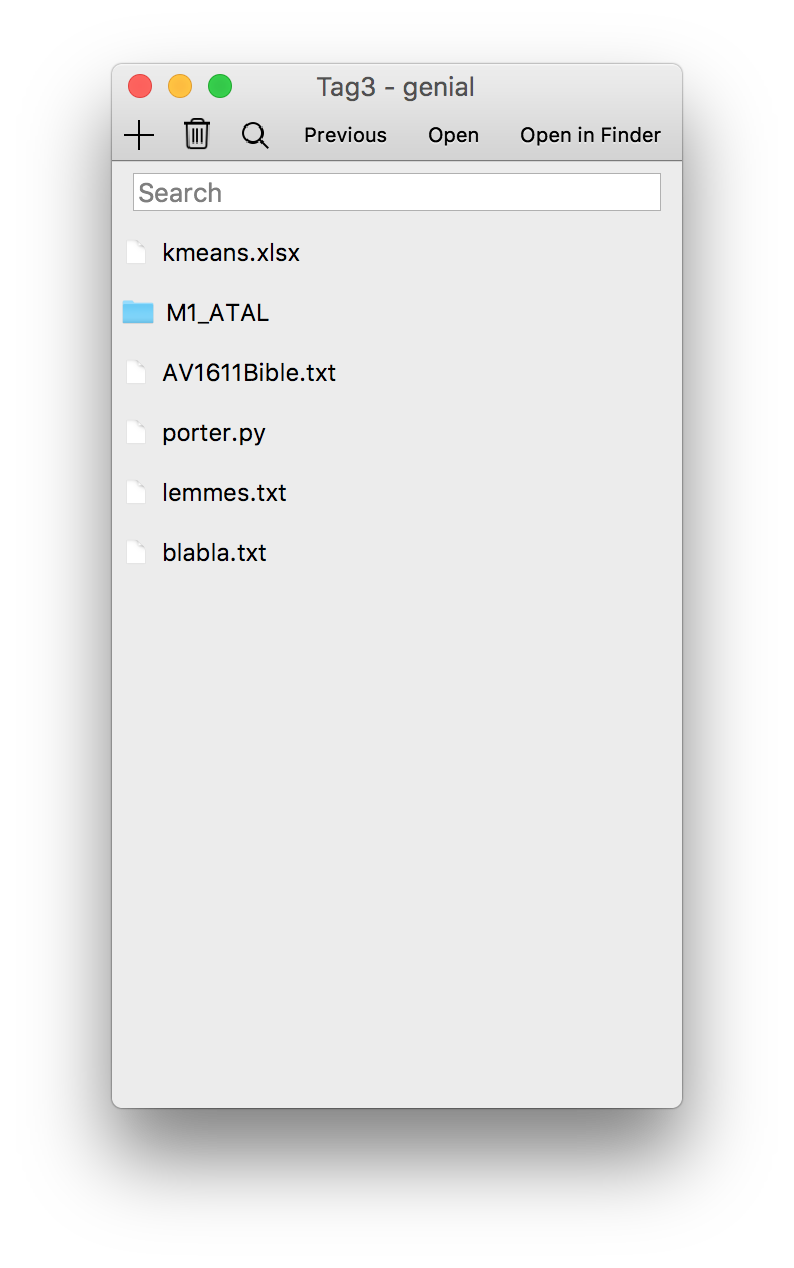
\includegraphics[width=4cm]{fichiersfiltre.png}
            \caption{Résultat du filtrage}
            \end{center}
        \end{figure}
    
    \section{Problèmes rencontrés et améliorations possibles}
    Pour aller plus loin, on pourrait transformer l'affichage de la liste des tags de manière à avoir des vraies zones de glisser déposer. On pourrait imaginer une présentation sous forme de tuiles selectionnables. \\
    Nous avons également pensé à hierarchiser les tags, en nous inspirant du système de libellés de Gmail qui permet de créer des sous-libellés. On aurait ainsi la possibilité de créer des sous-tags, par exemple pour avoir un tag "Musique" et un sous-tag "Intrumental".\\
    Nous n'avons aussi pas eu le temps d'implémenter le menu contextuel, qui peut s'avérer être une aide préciseuse pour certain-e-s utilisateur-trices\\
    Aussi, nous n'offrons la possibilité que de filtrer les tags en "union" de plusieurs tags, il serait intéressant de permettre de filtrer les tags par intersection ou exclusion.\\
    Enfin, pour aller plus loin dans l'intégration de notre application au système, il faudrait implémenter le raccourci Cmd+Z ou "Annuler" ainsi que le copier-coller à l'intérieur d'un tag, qui est un bon compromis entre l'ajout par navigation dans le système de fichier, qui est couteuse en nombre de clics et le glisser-déposer qui nécéssite d'avoir les fênetres au même plan. \\

\chapter{Conclusion}
    Nous avons réussi à aboutir à une application agréable à utiliser et fonctionnelle, même si celle-ci a encore des améliorations possibles. Notre but de départ était d'arriver à une application simple, minimaliste et assez bien intégrée à l'environnement de l'utilisateur-trice. Nous pensons avoir rempli cet objectif.

\end{document}
